\documentclass[
  bibliography=totoc,     % Literatur im Inhaltsverzeichnis
  captions=tableheading,  % Tabellenüberschriften
  titlepage=firstiscover, % Titelseite ist Deckblatt
]{scrartcl}
\newcommand{\pvec}[1]{\vec{#1}\mkern2mu\vphantom{#1}}
% Paket float verbessern
\usepackage{scrhack}

% Warnung, falls nochmal kompiliert werden muss
\usepackage[aux]{rerunfilecheck}

% unverzichtbare Mathe-Befehle
\usepackage{amsmath}
% viele Mathe-Symbole
\usepackage{amssymb}
% Erweiterungen für amsmath
\usepackage{mathtools}

% Fonteinstellungen
\usepackage{fontspec}
% Latin Modern Fonts werden automatisch geladen
% Alternativ zum Beispiel:
%\setromanfont{Libertinus Serif}
%\setsansfont{Libertinus Sans}
%\setmonofont{Libertinus Mono}

% Wenn man andere Schriftarten gesetzt hat,
% sollte man das Seiten-Layout neu berechnen lassen
\recalctypearea{}

% deutsche Spracheinstellungen
\usepackage{polyglossia}
\setmainlanguage{german}


\usepackage[
  math-style=ISO,    % ┐
  bold-style=ISO,    % │
  sans-style=italic, % │ ISO-Standard folgen
  nabla=upright,     % │
  partial=upright,   % ┘
  warnings-off={           % ┐
    mathtools-colon,       % │ unnötige Warnungen ausschalten
    mathtools-overbracket, % │
  },                       % ┘
]{unicode-math}

% traditionelle Fonts für Mathematik
\setmathfont{Latin Modern Math}
% Alternativ zum Beispiel:
%\setmathfont{Libertinus Math}

\setmathfont{XITS Math}[range={scr, bfscr}]
\setmathfont{XITS Math}[range={cal, bfcal}, StylisticSet=1]

% Zahlen und Einheiten
\usepackage[
  locale=EN,                   % deutsche Einstellungen
  separate-uncertainty=true,   % immer Fehler mit \pm
  per-mode=symbol-or-fraction, % / in inline math, fraction in display math
]{siunitx}

% chemische Formeln
\usepackage[
  version=4,
  math-greek=default, % ┐ mit unicode-math zusammenarbeiten
  text-greek=default, % ┘
]{mhchem}

% richtige Anführungszeichen
\usepackage[autostyle]{csquotes}

% schöne Brüche im Text
\usepackage{xfrac}

% Standardplatzierung für Floats einstellen
\usepackage{float}
\floatplacement{figure}{htbp}
\floatplacement{table}{htbp}

% Floats innerhalb einer Section halten
\usepackage[
  section, % Floats innerhalb der Section halten
  below,   % unterhalb der Section aber auf der selben Seite ist ok
]{placeins}

% Seite drehen für breite Tabellen: landscape Umgebung
\usepackage{pdflscape}

% Captions schöner machen.
\usepackage[
  labelfont=bf,        % Tabelle x: Abbildung y: ist jetzt fett
  font=small,          % Schrift etwas kleiner als Dokument
  width=0.9\textwidth, % maximale Breite einer Caption schmaler
]{caption}
% subfigure, subtable, subref
\usepackage{subcaption}

% Grafiken können eingebunden werden
\usepackage{graphicx}
% größere Variation von Dateinamen möglich
\usepackage{grffile}

% schöne Tabellen
\usepackage{booktabs}

% Verbesserungen am Schriftbild
\usepackage{microtype}

% Literaturverzeichnis
\usepackage[
  backend=biber,
]{biblatex}
% Quellendatenbank
\addbibresource{lit.bib}
\addbibresource{programme.bib}

% Hyperlinks im Dokument
\usepackage[
  unicode,        % Unicode in PDF-Attributen erlauben
  pdfusetitle,    % Titel, Autoren und Datum als PDF-Attribute
  pdfcreator={},  % ┐ PDF-Attribute säubern
  pdfproducer={}, % ┘
]{hyperref}
% erweiterte Bookmarks im PDF
\usepackage{bookmark}

% Trennung von Wörtern mit Strichen
\usepackage[shortcuts]{extdash}
%Grafiken an position H
\usepackage{float}
%immer noindent
\setlength\parindent{0pt}

\author{%
  Sinja Behrensmeier\\%
  \href{mailto:Sinja.Behrensmeier@tu-dortmund.de}{Sinja.Behrensmeier@tu-dortmund.de}%
  \texorpdfstring{\and}{,}%
  Yvonne Ribbeheger\\%
  \href{mailto:Yvonne.Ribbeheger@tu-dortmund.de}{Yvonne.Ribbeheger@tu-dortmund.de}%
  \texorpdfstring{\and}{,}%
  Lara Nollen\\%
  \href{mailto:Lara.Nollen@tu-dortmund.de}{Lara.Nollen@tu-dortmund.de}%
}
\publishers{TU Dortmund – Fakultät Physik}


\subject{Computational Physics}
\title{Übungsblatt 0}
\date{%
  Abgabe: 24.04.2020
}

\begin{document}

\maketitle
\thispagestyle{empty}
%\tableofcontents
\newpage

\section*{Aufgabe 0: Verständnisfragen}

\textbf{Frage 1): Was bedeutet numerische} Stabilität \textbf{und wieso tritt sie auf?}\\
Numerische Stabilität bedeutet, dass ein Verfahren stabil ist gegenüber kleinen Störungen der Daten. Die Ursache hierfür können beispielsweise Rundungsfehler sein, welche sich in jedem Verfahrensschritt verstärken. Ist ein Verfahren numerisch stabil, so werden sich die Fehler durch solche unvermeidbaren
Schwankungen durch das Verfahren nicht übersteigern. \\
\textbf{Frage 2): Wieso kann eine höhere} Genauigkeit \textbf{(beispielsweise durch feinere Diskretisierung) zu numerischer Instabilität führen?}\\
Bei feinerer Diskretisierung muss der Algorithmus häufiger angewendet werden, wobei der Fehler bei jedem Schritt verstärkt wird. Da nun mehr Schritte nötig sind, kann der Fehler auch stärker ansteigen und das Verfahren somit instabil werden. Auch können zusätzliche Terme, die bei einer Betrachtung mit höherer Genauigkeit hinzukommen und aufgrund von fehlerbehafteten Werten im Laufe des Verfahrens divergieren zu Instabilität führen.


\section*{Aufgabe 1: Distributivgesetz in der Floating Point-Arithmetik}
\textbf{Zu zeigen: Das Distributivgesetz }$(a\,\oplus\,b)\,\odot\,c\,=\,a\,\odot\,c\,\oplus\,b\,\odot\,c$\textbf{ ist in der Floating Point Arithmetik nicht mehr gültig, anhand eines Beispiels mit }$t\,=\,2$\textbf{ und }$l\,=\,1$.\\
Wähle: $a=1.0\cdot10^0$, $b=4.0\cdot10^{-2}$ und $c=3.0\cdot10^{0}$ \\
Dann gilt: $a\,\oplus\,b\,=1.04\cdot10^0\overset{\text{rd}}{\to}1.0\cdot10^0$, da die Mantissenlänge von 1.04 zu lang ist.
Damit ist $(a\,\oplus\,b)\,\odot\,c\,=1.0\cdot10^0\odot3.0\cdot10^0=3.0\cdot10^0$.\\
Auf der rechten Seite ergibt sich:\\$a\,\odot\,c\,\oplus\,b\,\odot\,c=3.0\cdot10^0\oplus1.2\cdot
10^{-1}=3.12\cdot10^{-2}\overset{\text{rd}}{\to}3.1\cdot10^{-2}\neq(a\,\oplus\,b)\,\odot\,c$

\section*{Aufgabe 2: Rundungsfehler}
\subsection*{Aufgabenteil a)}
Für große $x>>1$:
\begin{equation}
  f_a(x)=\frac{1}{\sqrt{x}}-\frac{1}{\sqrt{x+1}}
  \label{eqn:2amit}
\end{equation}
Die Funktion wird einmal direkt berechnet, was jedoch zur Auslöschung bei großen x führen kann, da in diesem Wertebereich $\frac{1}{\sqrt{x+1}}\approx \frac{1}{\sqrt{x}}$ gilt und es somit zu großen relativen Fehlern kommen kann. Daher kann auch ein alternativer Rechenweg gewählt werden, der dieses Problem vermeidet, indem die Funktion zunächst umgeschrieben wird:
\begin{align}
  \frac{1}{\sqrt{x}}-\frac{1}{\sqrt{x+1}}&=\frac{\sqrt{x+1}-\sqrt{x}}{\sqrt{x}\sqrt{x+1}} \\
  &=\frac{\sqrt{x+1}-\sqrt{x}}{\sqrt{x}\sqrt{x+1}}\cdot\frac{\sqrt{x+1}+\sqrt{x}}{\sqrt{x+1}+\sqrt{x}}\\
  &=\frac{x+1-x}{\sqrt{x}(x+1)+x\sqrt{x+1}}\\
  &=\frac{1}{\sqrt{x}(x+1)+x\sqrt{x+1}}=\tilde{f}_a(x)
  \label{eqn:2aohne}
\end{align}
Beide Berechnungsmethoden werden in einem Bereich von $x\in[10^5,10^7]$ verwendet um 10000 äquidistante
Datenpunkte zu generieren, wie in Abbildung \ref{fig:2a} doppellogarithmisch dargestellt ist.

\begin{figure}[H]
  \centering
  \includegraphics[height=8cm]{../plots/2a.pdf}
  \caption{Vergleich zwischen der Berechnung mit Auslöschung \eqref{eqn:2amit} und der Berechnung, welche Auslöschung vermeidet \eqref{eqn:2aohne}.}
  \label{fig:2a}
\end{figure}

Zwischen den beiden Rechenmethoden wird zudem die relative Abweichung gemäß der Gleichung
\begin{equation}
  \frac{\lvert f(x)-\tilde{f}(x)\rvert}{\lvert \tilde{f}(x) \rvert}
  \label{eqn:abw}
\end{equation}
berechnet, wie in Abbildung \ref{fig:2arel} dargestellt ist. Es ist zu erkennen, dass die ursprüngliche Funktion $f_a(x)$ stark um die umgestellte Funktion $\tilde{f}_a(x)$ schwankt, wobei letztere hingegen absolut stetig ist. Dies zeigt, dass durch das Umstellen der Formel die Auslöschung vermieden wird und die Ergebnisse für große Werte von $x$ somit deutlich exakter sind als ursprünglich. Dies lässt sich auch an der relativen Abweichung erkennen, welche im Schnitt für steigende Werte von $x$ stark ansteigt.

\begin{figure}[H]
  \centering
  \includegraphics[height=8cm]{../plots/2arel.pdf}
  \caption{Relative Abweichung zwischen den beiden Rechenmethoden aus Aufgabenteil a).}
  \label{fig:2arel}
\end{figure}

\subsection*{Aufgabenteil b)}
Für kleine $x<<1$:
\begin{equation}
  f_b(x)=\frac{1-\cos(x)}{\sin(x)}
  \label{eqn:2bmit}
\end{equation}
Auch hier kann es bei der direkten Berechnung zu Auslöschung kommen, da für kleine x: $\cos(x)\approx 1$ gilt.
Um dies zu vermeiden wird auch diese Formel zunächst umgestellt:

\begin{align}
  \frac{1-\cos(x)}{\sin(x)} &= \frac{1-\cos(x)}{\sin(x)}\cdot \frac{1+\cos(x)}{1+\cos(x)}\\
  &=\frac{1-\cos^2(x)}{\sin(x)(1+\cos(x))} \\
  &=\frac{\sin^2(x)}{\sin(x)(1+\cos(x))} \\
  &=\frac{\sin(x)}{(1+\cos(x))} =\tilde{f}_b(x)
  \label{eqn:2bohne}
\end{align}
Auch hier wurden je 10000 äquidistante
Datenpunkte in einem Bereich von $x\in[10^{-5},0.002]$ generiert, wie in Abbildung \ref{fig:2b} dargestellt ist.

\begin{figure}[H]
  \centering
  \includegraphics[height=8cm]{../plots/2b.pdf}
  \caption{Vergleich zwischen der Berechnung mit Auslöschung \eqref{eqn:2bmit} und der Berechnung, welche Auslöschung vermeidet \eqref{eqn:2bohne}.}
  \label{fig:2b}
\end{figure}

Die über Gleichung \eqref{eqn:abw} errechnete Abweichung zwischen beiden Verfahren ist in Abbildung \ref{fig:2brel} dargestellt. Dabei fällt auf, dass die ursprüngliche Funktion \eqref{eqn:2bmit} sprunghafte Anstiege zeigt wohingegen die Steigung der umgestellten Funktion \eqref{eqn:2bohne} kontinuirlich ist und somit
deutlich exaktere Werte liefert. Die Sprünge der ursprünglichen Funktion entstehen dabei auch hier durch Rundung und Auslöschung. In einem Bereich bis etwa $0.85\cdot10^{-2}$ liefert die Ursprungsfunktion sogar nur Werte von exakt 0, sodass die Abweichung in diesem Bereich 100\% beträgt. Bei höheren Werten lässt sich ein oszillierendes
Verhalten des relativen Fehlers erkennen, welcher jedoch insgesamt bei höheren Werten von $x$ stark abfällt, da sich hier $\cos(x)$ stärker von dem Wert 1 unterscheidet und Auslöschung somit eine nicht mehr so große Rolle spielt.


\begin{figure}[H]
  \centering
  \includegraphics[height=8cm]{../plots/2brel.pdf}
  \caption{Relative Abweichung zwischen den beiden Rechenmethoden aus Aufgabenteil b).}
  \label{fig:2brel}
\end{figure}

\subsection*{Aufgabenteil c)}
Für kleine $\delta<<1$:
\begin{equation}
  f_c(x)=\sin(x+\delta)-\sin(x)
  \label{eqn:2cmit}
\end{equation}
Auch hier kann es bei der direkten Berechnung zu Auslöschung kommen, da sich die beiden Sinus-terme nur geringfügig unterscheiden.
Somit ist es auch hier sinnvoll die Formel zunächst mithilfe der Additionstheoreme umzuschreiben:

\begin{align}
  \sin(x+\delta)-\sin(x) &=\sin(x)\cos(\delta)+\cos(x)\sin(\delta)-\sin(x) \\
  &= \cos(x)\sin(\delta) +\sin(x)(\cos(\delta)-1) \\
  &= \cos(x)\sin(\delta) + \frac{\sin(x)(\cos^2(\delta)-1)}{\cos(\delta)+1} \\
  &= \cos(x)\sin(\delta) - \frac{\sin(x)\sin^2(\delta)}{\cos(\delta)+1}=\tilde{f}_c(x)
  \label{eqn:2cohne}
\end{align}
Für die Variable $\delta$ wird ein Wert von $\delta=10^{-6}$ gewählt mit dem je 10000 äquidistante
Datenpunkte in einem Bereich von $x\in[0,4]$ generiert wird, wie in Abbildung \ref{fig:2c} dargestellt ist.

\begin{figure}[H]
  \centering
  \includegraphics[height=8cm]{../plots/2c.pdf}
  \caption{Vergleich zwischen der Berechnung mit Auslöschung \eqref{eqn:2cmit} und der Berechnung, welche Auslöschung vermeidet \eqref{eqn:2cohne}.}
  \label{fig:2c}
\end{figure}

Die relative Abweichung wird erneut über Gleichung \eqref{eqn:abw} berrechnet und ist in Abbildung \ref{fig:2crel} dargestellt. Auch hier ist ein Sprunghaftes Verhalten der ursprüngliche Funktion \eqref{eqn:2cmit} zu erkennen, wohingegen die umgestellte Formel eine kontinuierliche Kurve ergibt.
Auch der relative Fehler oszilliert immer wieder und zeigt einen Peak im Bereich von $x\approx\frac{\pi}{2}$, was daran liegt, dass die Funktion $\tilde{f}_c(x)$ in diesem Bereich Werte von $\tilde{f}_c(x)\approx 0$ annimmt und somit der Nenner in Gleichung \eqref{eqn:abw} divergiert.

\begin{figure}[H]
  \centering
  \includegraphics[height=8cm]{../plots/2crel.pdf}
  \caption{Relative Abweichung zwischen den beiden Rechenmethoden aus Aufgabenteil c).}
  \label{fig:2crel}
\end{figure}


\section*{Aufgabe 3: Stabilität}
\subsection*{Aufgabenteil a)}

Zur Lösung des Anfangswertproblems
\begin{equation}
  \.{y}(t)=-y(t),\quad y(0)=1
\end{equation}
wird in dieser Aufgabe zum einen das normale Eulerverfahren mit einer Schrittweite von
$\Delta t=0.1$ zur Diskretisierung implementiert sowie auch das symmetrische Eulerverfahren.
Die Rekursionsgleichung des normalen Eulerverfahrens ergibt sich dabei zu
\begin{equation}
  y_{n+1}=y_n(1-\Delta t)
\end{equation}
und die des symmetrischen Eulerverfahrens zu
\begin{equation}
  y_{n+1}=-2\Delta ty_n+y_{n-1} \: ,
\end{equation}
wobei bei letzterem zudem der Anfangswert $y_1=\text{exp}(-\Delta t)$ verwendet wird.
Die analytische Lösung dieses Problems lautet dabei
\begin{equation}
  y(t)=\text{exp}(-t) \: .
\end{equation}
Die resultierenden Werte im Bereich von $x\in[0,10]$ sind in Abbildung \ref{fig:Eulervergleich}
graphisch dargestellt. Es zeigt sich, dass das symmetrische Eulerverfahren numerisch instabil ist und daher bei großen $x$ stark um die analytische Lösung schwankt. Das normale Eulerverfahren ist hingegen numerisch stabil und zeigt nur eine vergleichsweise geringe Abweichung von der exakten Lösung.\\
\begin{figure}[H]
  \centering
  \includegraphics[height=8cm]{../plots/3_a.pdf}
  \caption{Vergleich des normalen Eulerverfahrens und des symmetrischen Eulerverfahrens mit der analytischen Lösung.}
  \label{fig:Eulervergleich}
\end{figure}
Dies lässt sich auch an den relativen Fehlern erkennen, welche sich über die Formel
\begin{equation}
  \frac{\lvert y_n-\text{exp}(-\Delta t \cdot n)\rvert}{\text{exp}(-\Delta t \cdot n)}
  \label{eqn:eulabw}
\end{equation}
ergibt und in Abbildung \ref{fig:eulerrel} dargestellt ist. Es lässt sich erkennen, dass der relative Fehler des
symmetrischen Eulerverfahren zunächst oszilliert und dann exponentiell ansteigt. Auch der relative Fehler
des normalen Eulerverfahrens steigt stetig an, jedoch weitaus langsamer als der des symmetrischen Eulerverfahrens.
\begin{figure}[H]
  \centering
  \includegraphics[height=8cm]{../plots/3rel_a.pdf}
  \caption{Relative Fehler des normalen und des symmetrischen Eulerverfahrens.}
  \label{fig:eulerrel}
\end{figure}


\subsection*{Aufgabenteil b)}

Im zweiten Aufgabenteil werden nun andere Anfangswerte gewählt, mit $y_0=1-\Delta t$ für das normale Eulerverfahren und für das symmetrische Eulerverfahren $y_0=1$ sowie $y_1=y_0-\Delta t$. Analog zu Aufgabenteil a) sind in Abbildung \ref{fig:Eulervergleich_b} die Ergebnisse der beiden Verfahren zusammen mit der analytischen Lösung dargestellt, sowie die relativen Fehler in Abbildung \ref{fig:eulerrel_b}.
\begin{figure}[H]
  \centering
  \includegraphics[height=8cm]{../plots/3_b.pdf}
  \caption{Vergleich des normalen Eulerverfahrens und des symmetrischen Eulerverfahrens mit veränderten Anfangswerten mit der analytischen Lösung.}
  \label{fig:Eulervergleich_b}
\end{figure}
\begin{figure}[H]
  \centering
  \includegraphics[height=8cm]{../plots/3rel_b.pdf}
  \caption{Relative Fehler des normalen und des symmetrischen Eulerverfahrens mit veränderten Anfangswerten.}
  \label{fig:eulerrel_b}
\end{figure}
Zur besseren Vergleichbarkeit beider Aufgabenteile sind die unterschiedlichen relativen Fehler zudem in
Abbildung \ref{fig:alle} gemeinsam dargestellt.
\begin{figure}[H]
  \centering
  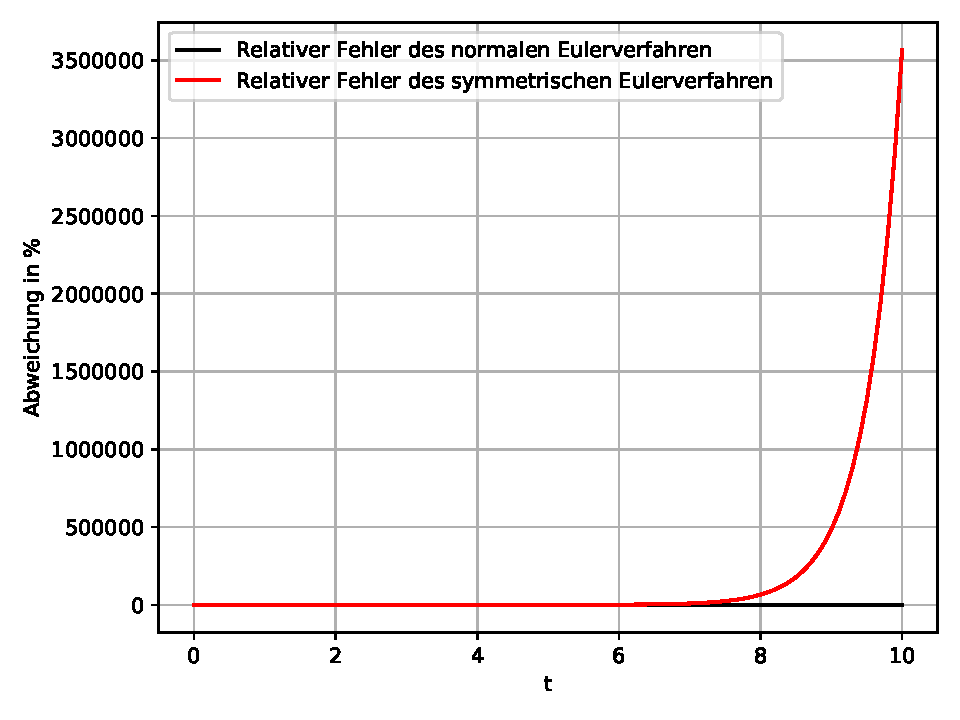
\includegraphics[height=8cm]{../plots/3rel.pdf}
  \caption{Relative Fehler des normalen und des symmetrischen Eulerverfahrens aus beiden Aufgabenteilen.}
  \label{fig:alle}
\end{figure}
Es lässt sich erkennen, dass sich für große $t$ die Fehler des normalen Eulerverfahrens kaum zwischen den beiden Aufgabenteilen unterscheiden und gegen denselben Wert konvergieren, was zu erwarten war, da das Verfahren numerisch stabil ist und der veränderte Anfangswert effektiv eine Verschiebung des Laufindex $n$ der Rekursion um einen Wert nach oben bedeutet, also $y_0\to y_1, y_1\to y_2$ usw. \\
Das symmetrische Eulerverfahren ist hingegen instabil, sodass bereis eine kleine Änderung des Anfangswertes
$y_1$ eine große Auswirkung auf das Ergebnis hat. Dadurch, dass $y_1$ in Aufgabenteil b) nicht mehr exakt mit dem analytischen Wert aus $y(t)=\text{exp}(-t)$ übereinstimmt, sind hier die Fehler bereits deutlich größer (Achtung: logarithmische Darstellung) und zeigen nicht so lange das oszillierende Verhalten, sondern zeigen schneller einen exponentiellen Anstieg.

\end{document}
